% !TEX root = ../phd-thesis.tex

\chapter{Under-approximation abstract domains}\label{ch:uai}
In this chapter, we try to use abstract interpretation for under-approximation analysis. In principle, the over-approximation theory can be dualized in an order-theoretic sense to obtain results for under-approximation. However, in this chapter we show that it is not so simple. Particularly, the semantics of basic constructs of the language are not dualized: therefore, the dual of an abstract domain that ``behaves well" with respect to basic transfer functions may not enjoy the same property.

We first point out some intuitive reasons that break the symmetry between over and under-approximation. Then, building on these observations, we formally derive some negative results showing that it is not possible to define Galois connection-based under-approximation abstract domains in a large class of instances. More in details, we assume that (i)~abstract analyses should return non-trivial results for large classes of programs and (ii)~to justify the convenience of the abstract analysis, the abstract domain should be significantly “smaller” than the concrete powerset. Under these assumptions, we prove that there is no under-approximation abstract domain able to analyse programs encoding certain classes of basic transfer functions.

The content of this chapter is based on~\cite{ABG22,ABG24}.

\section{Overview}
In their first work on Abstract Interpretation~\cite{CC77}, Patrick and Radhia Cousot introduced the formal theory that could be used to study both over and under-approximations.
However, while the former has been extensively studied, there are only sparse studies on under-approximation abstract domain.
For instance, Lev-Ami et al.~\cite{LSRG07} proposed to use complements of over-approximation domains to infer sufficient preconditions for program correctness. However, such an approach is severely limited in proving incorrectness, as we show in Example~\ref{ex:uai:complement-domain}.
For the same goal, Miné~\cite{Mine14} uses directly over-approximation domains, giving up the best abstraction and handling the choice of a maximal one with heuristics.
To infer necessary preconditions, Cousot et al.~\cite{CCL11,CCFL13} use abstract interpretation techniques but on Boolean formulas, hence bypassing the issue of defining an under-approximation abstract domain.
Schmidt~\cite{Schmidt07} uses higher-order domains, defining abstract states with the meaning ``there exists a value satisfying this over-approximation property'', hence giving rise to an under-approximation of over-approximations.
All the above approaches design under-approximation domains starting from over-approximation ones, and, to the extent of our knowledge, there are no abstract domains thought from the ground up for under-approximation program analysis.

We consider the problem of defining meaningful under-approximation abstract domains for program analysis over powerset concrete domains under the hypotheses (i) and (ii) above.
%\begin{figure}[t]
%	\centering
%	\begin{subfigure}{.5\textwidth}
%		\centering
%		{
%			\selectfont
%			\def\svgwidth{.8\textwidth}
%			\input{images/gc-intervals.pdf_tex}
%		}
%		\caption{Over-approximation intervals domain.}
%		\label{fig:uai:gc-intervals}
%	\end{subfigure}%
%	\begin{subfigure}{.5\textwidth}
%		\centering
%		{
%			\selectfont
%			\def\svgwidth{.8\textwidth}
%			\input{images/ugc-intervals.pdf_tex}
%		}
%		\caption{Under-approximation, complemented interval domain.}
%		\label{fig:uai:ugc-intervals}
%	\end{subfigure}
%	\caption{Example of complemented domain, using intervals.}
%	\label{fig:uai:gc-ugc-intervals}
%\end{figure}
From a purely mathematical point of view, this seems a trivial task because the theories of over and under-approximation are dual.
For instance, as done by Lev-Ami et al.~\cite{LSRG07}, we can transform any over-approximation domain into an under-approximation by reversing the order of its elements and complementing their interpretation. We call this construction \emph{complement domain}.
As an example, consider the (over-approximation) interval domain, where, e.g., the interval $[-1,1]$ is a correct abstraction for any subset of $\{ -1, 0, 1 \}$ and is the best abstraction of $\{ -1, 1 \}$ and $\{ -1, 0, 1 \}$. Instead, in the complement domain, the interval $[-1,1]$ is a correct abstraction of any set containing all values strictly smaller than $-1$ and all values strictly greater than $1$ and is the best abstraction of $\{ \dots, -3, -2, 0, 2, 3, \dots \}$ and $\{ \dots, -3, -2, 2, 3, \dots \}$. Note that, being an under-approximation, $[-1, 1]$ represents correctly any set \emph{larger} than its concretization $\{ \dots, -3, -2, 2, 3, \dots \}$.
However, we argue that complement domains are not useful for incorrectness analysis: in the above complement domain of intervals, initializations such as \code{i := 0} or \code{i := 1000} are abstracted to the interval $[-\infty,\infty]$, which is the best abstraction of any finite set but loses any information about the initial value of \code{i}. We give more details on complement domains in Example~\ref{ex:uai:complement-domain}.

Another important asymmetry we point out is the handling of divergence.
While it is not the only solution, it is common to represent divergence with the bottom element $\bot$ of the abstract domain. When doing so, this is case in both over and under-approximation. However, $\bot$ as an under-approximation also represents the absence of information; dually, in over-approximation this is described by $\top$. This is a problem since many concrete functions are strict, that is, when applied to a non-terminating expression, they also fail to terminate (they return $\bot$ if one argument is $\bot$), and, to be a correct under-approximation, also the corresponding abstract function needs to be strict:
\[
f^{\flat}(\bot) = f^{\flat}(\alpha(\emptyset)) \preceq \alpha(f(\emptyset)) = \alpha(\emptyset) = \bot
\]
This implies that whenever the analysis cannot determine any meaningful information at some program point, it has to propagate the absence of information along all program paths, at least until a join in the control flow is found.
So ``recovery'' from $\bot$, that is, producing a result different from $\bot$, once we start with it, is very hard in an under-approximation. On the contrary, ``recovery'' from $\top$ in over-approximation is easier: for example, this can happen whenever the code contains a constant assignment.

A last asymmetry we remark is that over-approximation abstract domains are closed under intersection, while under\hyp{}approximation abstract domains are closed under union. In the case of assignments this asymmetry has serious consequences. While the result of an assignment can be over-approximated by any larger set of values, with different degrees of precision, the only admissible under-approximations are either the singleton or the empty set. If not enough singletons are represented, then the under-approximation analysis is likely to give a trivial result. Conversely, if too many singletons are represented, closure under union will make the size of the under-approximation abstract domain grow exponentially, violating assumption (ii).

We further strengthen the asymmetry by using the concept of under-approximation Galois insertion (Definition~\ref{def:bg:under-gc}) to show how straightforward adaptations of some known over-approximation techniques do not work for under-approximation.
Then, we establish some negative results. The general theme is to fix some reasonable hypotheses over the common functions encoded by program fragments and then show that any under-approximate abstract domain with size not exponentially larger than the set of values (i.e., satisfying assumption (i)) will return no useful information for such program fragments.
Since the analysis is unable to recover from this lack of information, the result of the analysis of the entire program will be trivial (i.e., violating assumption (ii)).
Therefore, while any abstract domain for under-approximate reasoning may be effective for some carefully crafted programs, it will return trivial results on the majority of programs.

Formally, we first introduce the new definition of \emph{non-emptying function} (Definition~\ref{def:uai:non-emptying}), describing functions that do not tamper the analysis. Roughly speaking, a function on the concrete domain is non-emptying if it admits an under-approximation whose consecutive applications would not waste the analysis result by returning $\bot$.
Our first result proves that no abstract domain for integers can be constructed that makes all increments non-emptying. In other words, we prove that an analysis based on under-approximation domains would often report trivial information for programs that involve repeated increments. We do so both for the infinite domain $\pow(\setZ)$ and a finite integer domain $\pow([-N, N])$ for large $N$.

\begin{figure}[t]
	\begin{subfigure}{\textwidth}
		\centering
		\scalebox{0.93}{
			\begin{tabular}{c|ccc}
				Result                                              & Concrete domain & Tight hypotheses  & Generalizes                                         \\
				\hline
				Proposition~\ref{prop:uai:ne-sum-nonexsistence-inf} & $\pow(\setZ)$   & --                & --                                                  \\
				Theorem~\ref{th:uai:non-empt-res-local}             & $\pow(C)$       & High surjectivity & Proposition~\ref{prop:uai:ne-sum-nonexsistence-inf} \\
				Theorem~\ref{th:uai:non-empt-res-global}            & $\pow(C)$       & High surjectivity & Proposition~\ref{prop:uai:ne-sum-nonexsistence-inf} \\
			\end{tabular}
		}
		\caption{Tabular comparison of our results for infinite domains.}
		\label{fig:uai:tab-summary-infinite}
		\vspace{1ex}
	\end{subfigure}
	\begin{subfigure}{\textwidth}
		\centering
		\vspace*{0.5ex}
		\scalebox{0.93}{
			\begin{tabular}{c|cccc}
				Result                                              & Concrete domain & Tight hypotheses & Generalizes                                         & Inspired by                              \\
				\hline
				Proposition~\ref{prop:uai:ne-sum-nonexsistence-fin} & $\pow([-N, N])$ & --               & --                                                  & --                                       \\
				Theorem~\ref{th:uai:non-empt-res-finite-global}     & $\pow(C)$       & None             & Proposition~\ref{prop:uai:ne-sum-nonexsistence-fin} & Theorem~\ref{th:uai:non-empt-res-global} \\
			\end{tabular}
		}
		\caption{Tabular comparison of our results for finite domains.}
		\label{fig:uai:tab-summary-finite}
	\end{subfigure}
	\caption{Summary of the results in this chapter. The tables acts as a quick reference, showing which concrete domain they are applicable to, which of the hypotheses are (known to be) tight, and the relations between the results.}
\end{figure}

We then study how we can generalize these results to different concrete domains and function families.
We first focus on the case where the concrete domain is the powerset of an \emph{infinite} set of values, and we prove two results, one local and one global, for infinite concrete domains. To do so, we introduce the notion of \emph{highly surjective function family} (Definition~\ref{def:uai:highly-onto-func-family}), of which sums are an instance. The local condition applies to each function in the family, while the global condition is a property of the whole family. Contrary to the definition of non-emptying functions, the notion of highly surjective function family is independent of the abstract domain. Once again the main consequence of our results is that abstract analyses of programs involving the application of functions in the family will often report trivial information. As in the case of increments, highly surjective function families are commonly coded in programs.
Finally, we show that the hypothesis of high surjectivity is tight by presenting mathematical constructions of abstract domains making all functions in a family non-emptying.
Our results for infinite domains are summarized in Table~\ref{fig:uai:tab-summary-infinite}: both results for an arbitrary infinite set $C$ generalize the result for integers. The hypothesis of high surjectivity is tight, but we do not know about all the others.

Lastly, we focus on the powerset of a \emph{finite} set of values. We discuss why a straightforward adaptation of the two results for the infinite case to the finite one was not possible, most notably a difference with the very definition of highly surjective function family. We then propose a general result for this case, inspired by the global condition for the infinite case, but whose details are different.
Our results for finite domains are summarized in Table~\ref{fig:uai:tab-summary-finite}: our single result generalizes again the result for integers, but we were not able to prove any of our hypotheses tight.

\section{Comparison with over-approximation}\label{sec:uai:examples}
We revisit some known over-approximation analyses and techniques, showing how specific characteristics of under-approximation makes this a challenging task.

\subsection*{Complement domain}
The first attempt, already briefly discussed in the introduction, is the use of the complement of an over-approximation abstract domain. This is an application of the order theoretic duality, but it turns out the resulting domains are not often useful for analysis. For instance, for domains already closed under complementation (eg. the Sign domain) this construction yields the same domain. However, this is not the case in general.

\begin{example}[Complement domain]\label{ex:uai:complement-domain}
	Whenever the concrete domain is a powerset $\pow(C)$, we can exploit the complement $\lnot : \pow(C) \rightarrow \pow(C)$ to define a UGC from any given GC by taking complements of the concretization. Formally, given a GC $\gc{\pow(C)}{\alpha}{\gamma}{A}$, then $\ugc{\pow(C)}{\alpha \circ \lnot}{\lnot \circ \gamma}{A^{\op}}$ is a UGC (this stems from $\lnot : \pow(C) \rightarrow \pow(C)^{\op}$ being an isomorphism of posets).
	For instance, given the interval domain, we can define its complement by
	\[
	\gamma_{\lnot}([n, m]) = \lnot \gamma([n, m]) = \setZ \setminus \{ x \in  \setZ \svert n \le x \le m \} = \{ x \in \setZ \svert x < n \lor m < x \}
	\]
	The set of abstract elements is the same as $\Int$, but the ordering is reversed, so we call this domain $\Int^{\op}$. The (under-approximation) Galois Connection with $\pow(\setZ)$ is given by $\gamma_{\lnot} = \lnot \circ \gamma$ and $\alpha_{\lnot} = \alpha \circ \lnot$. Note that, thanks to the ordering in $\Int^{\op}$ being the opposite, both $\alpha_{\lnot}$ and $\gamma_{\lnot}$ are monotone.

	While $\Int^{\op}$ is a sound under-approximation abstract domain, we argue that it is not useful for incorrectness analysis. Consider a command as simple as the initialization \code{i := 0} that may happen at the beginning of a loop. This requires the analysis to abstract the concrete element $\{ 0 \}$, the set of values \code{i} may assume at the beginning of the loop. According to the above definition, we have
	\[
	\alpha_{\lnot}(\{ 0 \}) = \alpha(\lnot \{ 0 \}) = \alpha(\setZ \setminus \{ 0 \}) = [-\infty, +\infty]
	\]
	that is the bottom element of $\Int^{\op}$ since the ordering is reversed. We can better understand the reason for getting bottom by recalling that the meaning of an interval in $\Int^{\op}$ is the set of elements that are \emph{not} in the interval:
	\[
	\gamma_{\lnot}([-\infty, +\infty]) = \lnot \gamma([-\infty, +\infty]) = \lnot \setZ = \emptyset
	\]
	Other than the intuition that we lost all the information about the initialization, since $[-\infty, +\infty]$ is $\bot$ the analysis incurs in the issue described in the Overview about ``recover'' from $\bot$, effectively making the analysis unable to infer anything.

	This line of reasoning can be generalized to any finite concrete set $X$: $\setZ \setminus X$ is not bounded, as it contains all integers greater than $\max(X)$ and smaller than $\min(X)$ (which are both finite), so its abstraction through $\alpha$ is $[-\infty, +\infty]$.
\end{example}

\subsection*{Compositionality}
An important property of Abstract Interpretation analysis is compositionality. However, citing O'Hearn~\cite[§8]{OHearn20}, ``for incorrectness reasoning, you must remember information as you go along a path [...]''. This means that a compositional under-approximation analysis must be precise enough to have locally all the informations which should be carried over to the next piece of code. Over-approximation instead is way less restrictive in this sense, since ``for correctness reasoning, you get to forget information as you go along a path'' (O'Hearn~\cite[§8]{OHearn20}). As an example, we present dependency analysis, which is compositional for over-approximation but it is not for under-approximation.

\begin{example}[Dependency analysis]
	A dependency analysis (e.g.,~\cite[\S 6]{ANSTT17}) aims to compute, for each variable at every program point, the set of values it depends on. They are used for instance to check security properties such as information flow constraints.

	The result of the analysis is usually expressed with a collection of atomic dependencies $x \rightsquigarrow y$, meaning that the \emph{current} value of $y$ depends on the \emph{initial} value of $x$.
	For instance, consider the code
	\[
	\code{if (x == pwd) \{ y = y + 100 \}; x:= 0}
	\]
	The analysis of this fragment returns the dependencies $x \rightsquigarrow y$, $y \rightsquigarrow y$, as the final value of $y$ depends on the initial values of both $x$ and $y$. Note that the analysis does not compute any dependency with $x$ on the right as the final value of $x$ is always $0$, hence it carries no dependency.

	Over-approximation dependency analysis heavily exploits \emph{transitivity} (as it enables compositional reasoning): if $C_1$ exhibit the dependency $x \rightsquigarrow y$ and $C_2$ exhibits $y \rightsquigarrow w$, then $C_1 \code{;} C_2$ \emph{may} induce $x \rightsquigarrow w$. As a trivial example, $\code{y := x; w := y}$ yields the dependency $x \rightsquigarrow w$.
	However, transitivity is not well-behaved for under-approximation, whose goal is to find true dependencies only. The issue is that dependencies may cancel each other when composed. As a simple example, consider the code
	\begin{align*}
		C_1 & = \code{y := x; z := -x} \\
		C_2 & = \code{w := y + z}
	\end{align*}
	An under-approximation dependency analysis for $C_1$ may return $x \rightsquigarrow y$ and $x \rightsquigarrow z$ because they are true dependencies. Similarly, for $C_2$ it could deduce $y \rightsquigarrow w$. However, for the composition $C_1 \code{;} C_2$ the transitive inference $x \rightsquigarrow y \rightsquigarrow w$ isn't sound because $w$ is always $0$, so it doesn't depend on anything.
\end{example}

\subsection*{Closure under union}
Lastly, we consider non-relational analyses. Intuitively, a non-relational analysis cannot capture relationships between different variables. However, under-approximation cannot forget information along a path, including precise relations between variables. This means that non-relational domains cannot be used for under-approximation.
% Note that the complement of a non-relational abstract domain, constructed as in Example~\ref{ex:uai:complement-domain}, is relational.

\begin{example}[Non-relational domain]
	Informally, a non-relational abstract domain is a tuple of elements, one for each variable $x$, and describes the set of concrete states where each variable belongs to the values in its abstract coordinate. The abstraction is performed on each variable independently, projecting all states in $S$ on that variable and then abstracting the resulting set. The concretization is performed on each variable independently, and then the results are combined in all possible ways to get concrete values.

	As an example, consider the product of one interval domains for each variable. For instance, take the code
	\[
	\code{y := 5 - x; z := x + y}
	\]
	and assume at the beginning the variable \code{x} assumes values in the interval $[0, 3]$. An interval analysis on this fragment would find that \code{y} takes values in the interval $5 - [0, 3] = [2, 5]$, and then \code{z} is in the result of $[0, 3] + [2, 5] = [2, 8]$. However at the end of the program \code{z} is always $5$, so this is a sound over-approximation but is not as precise as it can be.
	The issue here is that the values of \code{x} and \code{y} are not independent, so an operation between these two variables cannot actually receive all possible inputs with \code{x} in $[0, 3]$ and \code{y} in $[2, 5]$, but just those that also satisfy the \textit{relationship} \code{y = 5 - x}. However, the interval domain knows nothing about this relationship since it abstracts each variable independently. More precisely, the possible pair of values for $x, y$ are $\{ (0, 5), (1, 4), (2, 3), (3, 2) \}$, but the abstraction is computed projecting on one variable (for instance $x$) and then computing the interval over-approximating that set (so that the abstraction for $x$ is $[0, 3]$). Then, the concretization contains all the pairs in the product $[0, 3] \times [2, 5]$, which are much more.

	\begin{figure}[t]
		\centering
		{
			\fontsize{11pt}{13pt}\selectfont
			\def\svgwidth{3in}
			\input{images/non-rel-proof.pdf_tex}
		}
		\caption{Non-relational domains are not closed under union}
		%\Description{The figure shows two rectangles in the Cartesian plane, corresponding to the concretization of two different abstract points in a non-relational domain. In the example, the union of the rectangles is not a rectangle, therefore it cannot be the concretization of a third abstract point.}
		\label{fig:uai:rel-domain}
	\end{figure}
	In general, this projection is not sound for under-approximation: the concretization is not able to recover which of the original pairs were in the concrete set and which were not. On a more abstract level, such a domain is not closed under union: elements of the abstract domain are ``rectangles'' in the Cartesian plane with variables on the axes (since they are concretized to the Cartesian product of the abstractions for each variable) and the union of rectangles is not a rectangle. This is shown in Figure~\ref{fig:uai:rel-domain}: the union of the light and dark rectangles is not a rectangle as it misses the top-left ``corner''.
\end{example}

\section{Non-emptying functions}\label{sec:uai:non-emptying}
A central concept in our development is the following definition of \emph{non-emptying function}. To understand the rationale behind it, recall that $\bot$ means no information in the under-approximation setting, while any other abstract value is ``something'' interesting.
\begin{definition}[Non-emptying function]\label{def:uai:non-emptying}
	Let $\ugc{C}{\alpha}{\gamma}{A}$ be a UGC, $f : C \rightarrow C$ a monotone function and $f^{A} = \alpha \circ f \circ \gamma$ its bca.
	We say that $f$ is \emph{non-emptying} (in $A$) if, for any concrete value $c$, $\alpha(c) \neq \bot$ and $\alpha(f(c)) \neq \bot$ imply $f^{A}(\alpha(c)) \neq \bot$.
\end{definition}
The idea behind this definition is that if the analysis starts from something meaningful ($\alpha(c) \neq \bot$) and it can find something significant ($\alpha(f(c)) \neq \bot$) then it will find at least one of the possible results ($f^{A}(\alpha(c)) \neq \bot$), thus not degrading the result of the analysis to $\bot$ and avoiding the issues discussed above. Intuitively, we want basic transfer functions to be non-emptying so that their analysis doesn't return $\bot$. Note that this idea is tailored to forward analysis \todo{Say forward analysis at the beginning}. The following toy example illustrates the meaning of the definition.
\begin{example}\label{ex:uai:non-ne-impair-analysis}
	Consider the simple imperative fragment
	\[
	\code{if (x $\neq$ 0) then \{ while (x < 10) \{ y := 7 / x; x := x + 1; \} \}}
	\]
	where a careless programmer used the condition \code{x $\neq$ 0} instead of the expected \code{x > 0}: on any initial state where $x$ is negative the program incurs a division by $0$ error.

	For the analysis, suppose \code{x} is an integer value and consider the domain $\Int_{01} = \{ I \in \Int \svert 0 \in I \lor 1 \in I \} \cup \{ \bot \}$, a variation of $\Int_0$ from Example~\ref{ex:bg:intervals0} such that each interval in $\Int_{01}$ must contain at least one of $0$ and $1$.
	By an argument similar to that for $\Int_0$ it can be shown that $\Int_{01}$ is closed under union (since $0$ and $1$ are consecutive values in the integer domain), and thus is an under-approximation domain, whose abstraction function maps each set of integers to the largest interval that is included in the set and that contains $0$ or $1$.

	In this domain, the semantics $f$ of the increment $x := x + 1$ is not non-emptying: for instance, on the concrete value $c = \{-1, 1, 2, \dots, 10 \}$ we have $\alpha(c) = [1, 10] \neq \bot$ and $\alpha(f(c)) = \alpha(\{ 0, 2, 3, \dots, 11 \}) = [0] \neq \bot$ but $f^A(\alpha(c)) = f^A([1, 10]) = \alpha(f(\gamma([1, 10]))) = \alpha(\{ 2, 3, \dots, 11 \}) = \bot$. We show in the following the effect of this on the analysis.

	Assume to start the analysis in this domain with the initial condition $[-1, 10]$ for variable $x$: remember that this being an under-approximation analysis, the abstract state $[-1, 10]$ means that $x$ may assume all the values in that interval at the beginning of the code fragment.
	In the concrete execution, the filter $x\neq 0$ then produces the concrete set of values $c = \{-1, 1, 2, \dots, 10 \}$, but the abstract interpreter must abstract this to its largest subset that is an interval containing $0$ or $1$, that is $[1, 10]$. The abstract analysis of the cycle then proceeds straightforwardly, finding $\bot$ after one iteration of the loop body (since after the increment the set of values for $x$ is $\{2, 3, \dots, 11 \}$ that is abstracted to $\bot$ because it contains neither $0$ nor $1$) and so the abstract fixpoint of the loop is the interval $[1, 10]$.
	This yields no error, even though the concrete execution starting at $x = -1$ does indeed fail after one iteration.
\end{example}

For the remainder of the paper, we assume to be given a set of \emph{values} $C$ and a UGI $\ugi{\pow(C)}{\alpha}{A}$ whose concrete domain is $\pow(C)$.
In the following, we present the basic technical tools we use to prove our theorems (Propositions~\ref{prop:uai:ne-sum-nonexsistence-inf}, \ref{prop:uai:ne-sum-nonexsistence-fin} and Theorems~\ref{th:uai:non-empt-res-local}, \ref{th:uai:non-empt-res-global}, \ref{th:uai:non-empt-res-finite-global}), which all follows the same pattern. First we make the assumption that the abstract domain is not \emph{too large} to hinder the analysis, but then we show that if all the functions in a given family were non-emptying, the abstract domain would grow too large.
Particularly, we start from a representable element (which is assumed to exist by hypothesis), then use Lemma~\ref{lmm:uai:f-non-repr-pair} to build other representable elements, up until the size of the abstract domain blows up. To get this, we exploit an exponential increase in the size of $A$ caused by ``closure under union'', that is the fact that if two concrete elements are representable in the abstract domain, their union is representable as well.

\begin{definition}\label{def:uai:repr-with-set}
	Let $S \subseteq C$ be a subset of $C$, and $\ugi{\pow(C)}{\alpha}{A}$ is an a UGI. We say that $d \in C$ is \emph{representable with $S$} if $S \cup \{ d \}$ is representable in $A$, ie. $\alpha(S \cup \{ d \}) = S \cup \{ d \}$. We call $R_A(S)$ the set of elements of $C$ representable with $S$, i.e.
	\[
	R_A(S) = \{ d \in C \svert \alpha(\{ d \} \cup S) = \{ d \} \cup S \}
	\]
\end{definition}

For the sake of brevity, we omit the subscript $A$ whenever it is clear from the context, we write $R$ for $R(\emptyset)$, the set of representable values of $C$, and use the shorthand $R(c)$ for $R(\{ c \})$ when $c \in C$ is a concrete value.
The following lemma, valid for non-emptying functions, explains the role played by Definition~\ref{def:uai:non-emptying} in proving all our negative results. Roughly speaking, it states that for $f$ to be non-emptying, some concrete values must be representable in the abstract domain.

\begin{lemma}\label{lmm:uai:f-non-repr-pair}
	Let $f: C \rightarrow C$ be non-emptying, $c \in R$ and $\tilde{c} \notin R(c)$. If $f(\tilde{c})\in R$, then $f(c) \in R$.
\end{lemma}

While the broad outline of all of our theorems is always the same, they differ in how they solve two key issues: first, it must be possible to apply Lemma~\ref{lmm:uai:f-non-repr-pair}; second, all the new representable elements obtained by applying it must be different from one another. In the following, we present various sets of conditions that can guarantee these two points, hence getting hypotheses for non existence of under-approximation abstract domains.

\section{Integer domains}\label{sec:uai:integer}
In this section, we apply the idea from the previous section on the concrete domain of integers and prove that any under-approximation abstract domain will likely return trivial analyses for programs that include sums inside arithmetic expressions.

\subsection{Infinite integer domain}\label{sec:uai:integers-infinite}
As a first example, we consider the infinite domain $\pow(\setZ)$ over all integers.
\begin{assump}\label{assump:uai:size-A-infinite-integers}
	We assume that an abstract domain $A$, to be feasible for analyses, must be at most countable.
\end{assump}
We make this assumption because we want the analysis to have a complexity comparable to that of a single concrete execution: if the analysis could be as complex as an arbitrary set of concrete executions, we could use those instead of the abstract domain. Therefore, we require the abstract domain to have the same size of the set $\setZ$ of values handled by the program, and not the concrete domain $\pow(\setZ)$. Many abstract domains, such as intervals, octagons~\cite{Mine06} and polyhedrons~\cite{CH78} with at most $n$ edges, satisfy it; some, such as general polyhedrons, do not, but indeed they also exhibit a worst-case exponential cost.

Based on Assumption~\ref{assump:uai:size-A-infinite-integers}, we prove a simple cardinality estimate that is exploited to prove that there are few representable elements.
\begin{lemma}\label{lmm:uai:R-S-bound-integer-inf}
	For any fixed subset $S \subseteq \setZ$, $R(S)$ is finite.
\end{lemma}
The result for integers now shows that no under-approximation abstract domain makes all sums non-emptying. The idea of the proof is to define an infinite sequence of representable elements, which is in contradiction with the previous lemma that says that $R = R(\emptyset)$ is finite.
To define such a sequence, we want to use Lemma~\ref{lmm:uai:f-non-repr-pair}: we start from an initial representable $n_0$ and from a value $\bar{n}$ not representable with it, then find a non-emptying $f$ that maps $\bar{n}$ into $n_0$, so that $f(\bar{n})$ is representable and we can then apply the lemma to get the new representable element $f(n_0)$. We then iterate this procedure, changing $f$, to build the infinite sequence.
We believe the hypothesis that there exists an initial representable value is not very restrictive since initializations like \code{x = 0} must be abstracted to $\bot$ if $0$ is not representable.
\begin{prop}\label{prop:uai:ne-sum-nonexsistence-inf}
	Let $\ugi{\pow(\setZ)}{\alpha}{A}$ be a UGI, and assume that there is an integer $n_0$ that is representable. Then it cannot be the case that all the functions of the form $f_n(x) = x + n$ are non-emptying in $A$.
\end{prop}
\begin{proof}%[Proof of Proposition~\ref{prop:uai:ne-sum-nonexsistence-inf}]
	Towards a contradiction, let us assume that all $f_n$ are non-emptying in $A$.
	By hypothesis, $n_0 \in R$ and $R(n_0)$ is at most finite by Lemma~\ref{lmm:uai:R-S-bound-integer-inf}. Since $\setZ$ is infinite, there exists an $\bar{n} \in \setZ \setminus (R(n_0) \cup \{ n_0 \})$, that is $\bar{n}$ is an element such that the pair $\{ n_0, \bar{n} \}$ is not representable.
	Let $d = n_0 - \bar{n}$, and let us prove by induction on $t$ that $n_0 + t d$ is representable for all $t$. The base case $t = 0$ is the hypothesis that $n_0$ is representable. For the inductive case, assume $n_0 + t d$ is representable, and consider the non-emptying function$f_{(t+1) d}$. We get:
	\begin{equation*}
		f_{(t+1) d}(\bar{n}) = \bar{n} + (t+1) d = \bar{n} + n_0 - \bar{n} + t d = n_0 + t d
	\end{equation*}
	that is representable by inductive hypothesis.
	By the instance of Lemma~\ref{lmm:uai:f-non-repr-pair} for the pair $\{ n_0, \bar{n} \}$ and the function $f_{(t+1) d}$, we get that $f_{(t+1) d}(n_0) = n_0 + (t+1) d$ is representable too, that is exactly the inductive step.

	Since $\bar{n} \neq n_0$ also $d \neq 0$, hence $\{ n_0 + t d \svert t \in \setN \}$ is infinite.
	Moreover $\{ n_0 + t d \svert t \in \setN \} \subseteq R$ by the induction above, but this is impossible since $R$ must be finite by Lemma~\ref{lmm:uai:R-S-bound-integer-inf}.
\end{proof}
The meaning of this proposition for program analysis is the fact that a domain small enough (by Assumption~\ref{assump:uai:size-A-infinite-integers}) is probably unable to deduce meaningful information on an integer domain: if it does not contain representable singletons it must abstract to $\bot$ any variable initialization, and otherwise, it cannot be non-emptying for all sums, hence getting $\bot$ when values are manipulated using this operation. In both cases, because of strictness, the abstract $\bot$ is propagated along program paths, yielding it as the final result of the analysis, which means exactly it cannot determine any information. This issue is not bound to manifest for all programs, but for any domain there exist programs for which it does.

Note that the only hypothesis on the abstract domain is related to its size, by Assumption~\ref{assump:uai:size-A-infinite-integers}. This would include all classical numerical domains such as intervals, octagons or congruences~\cite{Granger91}. Of course, these are over-approximation domains, so this result does not apply to them, but it shows that our hypotheses are very general and would include many known abstract domains.

\subsection{Finite integer domain}\label{sec:uai:integers-finite}
An analogous result can be obtained for a finite integer domain $\pow([-N, N])$, where $N$ is some large integer. This concrete domain models machine integers, that are constrained within an interval, so we assume that operations are performed in machine arithmetic, that is wrapping around in case of overflows. This is modelled working modulo $2N + 1$, the length of the interval, and taking the unique representative of each congruence class in the interval $[-N, N]$ of interest. It is worth noting that we take an interval that is symmetric around $0$ to simplify notation, but there is no conceptual difference in using an asymmetric one instead (eg. $[-N -1; N]$ to be closed under two's complement).
\begin{assump}\label{assump:uai:size-A-finite-integers}
	We assume that an abstract domain $A$, to be feasible for the concrete domain $\pow([-N, N])$, must have a cardinality that is polynomial in $N$.
\end{assump}
This assumption, just like Assumption~\ref{assump:uai:size-A-infinite-integers}, guarantees that for any set of input values the cost of the analysis is always polynomial in that of a single concrete execution, while the concrete analysis could require an exponential cost.

In the following, we use asymptotic notation for some quantities. Therefore, for each $N$ we consider the concrete set of values $C_N = [-N, N]$ and define an abstract domains $A_N$ for the concrete domain $\pow([-N, N])$. Intuitively, each $A_N$ represents the same abstraction, just instantiated for different values of $N$. With this notation, Assumption~\ref{assump:uai:size-A-finite-integers} becomes $\abs{A_N} = O(\text{poly}(N))$.

The next lemma is analogous to Lemma~\ref{lmm:uai:R-S-bound-integer-inf} in proving that some sets are small under Assumption~\ref{assump:uai:size-A-finite-integers} on the cardinality of $A_N$. Here, the ``exponential increase'' we mentioned is explicit, as we are dealing with finite quantities. For brevity, we write $R_N$ instead of $R_{A_N}$.
\begin{lemma}\label{lmm:uai:R-S-bound-integer-fin}
	Let $S \subseteq [-N_0, N_0]$ for some $N_0$. Then, $\abs{R_{N}(S)} = O(\log(N))$.
	%	Fixed a set $S$ that, for some $N_0$, is a subset $S \subseteq [-N_0, N_0]$, we have $\abs{R_{N}(S)} = O(\log(N))$.
\end{lemma}
The following proposition uses the same proof line as Proposition~\ref{prop:uai:ne-sum-nonexsistence-inf} above: we define a sequence of representable elements and prove that they are too many since, by the previous lemma, $R_N$ is quite small.
\begin{prop}\label{prop:uai:ne-sum-nonexsistence-fin}
	Let $\ugi{\pow([-N, N])}{\alpha}{A_N}$ be a UGI for all $N$, and assume that there is an integer $n_0$ that is representable in all the $A_N$. Then there exists an $N_0$ such that, for all $N > N_0$, it cannot be the case that all the functions of the form $f_n(x) = x + n$ (modulo $2N + 1$) are non-emptying in $A_N$.
\end{prop}
\begin{proof}
	Let $r_N = \abs{R_N(n_0)}$. By the previous Lemma~\ref{lmm:uai:R-S-bound-integer-fin} we know that $r_N = O(\log(N))$. For all $N$, fix an element $\bar{n}_N \notin R_N(n_0)$ not representable with $n_0$ in $A_N$ such that $d_N = n_0 - \bar{n}_N \le r_N + 1$.
	This element exists because otherwise all elements in the interval $[n_0 - r_N - 1, n_0 - 1]$ (modulo $2N + 1$) would be representable with $n_0$, that is impossible since that interval contains $r_N + 1 = \abs{R_N(n_0)} + 1$ elements.

	Consider an $N$ such that all the functions of the form $f_n(x) = x + n$ (modulo $2N + 1$) are non-emptying in $A_N$.
	Following the proof of Proposition~\ref{prop:uai:ne-sum-nonexsistence-inf}, we can show by induction on $t \ge 1$ that the value $f_{t d_N}(\bar{n}) = n_0 + (t - 1) d_N$ is representable in $A_N$. All these values are different from one another for
	\begin{equation*}
		1 \le t < \frac{2N + 1}{d_N}
	\end{equation*}
	so that
	\begin{equation*}
		\abs{R_N} \ge \frac{2N + 1}{d_N}
	\end{equation*}
	However, we know that $\abs{R_N} = O(\log(N))$ and $(2N + 1) / d_N = \omega(\log(N))$, therefore there exists some $N_0$ such that for any $N > N_0$ this inequality does not hold. This in turn implies that for all $N > N_0$ it is not possible that all the functions of the form $f_n(x) = x + n$ (modulo $2N + 1$) are non-emptying in $A_N$.
\end{proof}

Again, the only assumption on $A_N$ is about its size, so our result applies to many kinds of domains. For instance, a predicate abstraction \cite{GS97} with $\Omega(\log(N))$ predicates exceeds this bound, as its size is doubly exponential in the number $n$ of predicates.

\section{General infinite concrete domains}\label{sec:uai:infinite}
In this section, we try to extend the results of the previous Section~\ref{sec:uai:integers-infinite} on the infinite concrete domain of integers to other infinite concrete domains. More precisely, we deal with an infinite set $C$ of concrete values, and a UGI $\ugi{\pow(C)}{\alpha}{A}$.
Again, we take the Assumption~\ref{assump:uai:size-A-infinite-integers} on the size of $A$.
Under this assumption, we can prove again Lemma~\ref{lmm:uai:R-S-bound-integer-inf}, that does not depend on the specific integer domain considered in the previous section.

All conditions we propose in this section are mainly on the family of functions considered and not on the abstract domain. The reason for this is that first we fix a function family, corresponding to a program, and then we look for a domain well suited to analyse the specific family at hand. In other words, the family is given by the applicative context, while the domain can be adapted to it.

\begin{definition}[Highly surjective function family]\label{def:uai:highly-onto-func-family}
	Given a family $F$ of functions from $C$ to itself and an element $c \in C$, let
	\[
	P_F(c) = \{ d \in C \svert \exists f \in F .\ f(d) = c \}
	\]
	be the set of \emph{preimages of $c$}, elements of $C$ that can be mapped to $c$ by a function in $F$.
	We say that the family $F$ is \emph{highly surjective} if $P_F(c)$ is infinite for any possible choice of $c \in C$.
\end{definition}
This property is needed together with Lemma~\ref{lmm:uai:R-S-bound-integer-inf} to apply Lemma~\ref{lmm:uai:f-non-repr-pair} and get a new representable element: since there are infinitely many preimages of $c$ but $R(c)$ is finite, there are elements $\tilde{c} \in P_F(c)$ not in $R(c)$; then by definition of $P_F(c)$ there is an $f$ such that $f(\tilde{c}) = c \in R$, so we can apply the lemma to get $f(c) \in R$.
The reason for requiring $f(\tilde{c}) = c$ instead of just in $R$ is that, at the beginning of the proof, we assume $R$ to contain only one element, hence the two conditions are equivalent.
Starting from this basic idea, we present two sets of sufficient conditions to prove the non existence of any under-approximation abstract domain.

\subsection{Local requirements for impossibility}
The first set of conditions we propose is in a sense more ``local'', in that it requires conditions on each function in the family $F$, independently of the others.

The proof of this result proceeds as follows: it starts from a representable $c_0 \in R$ and iteratively creates an infinite sequence $\{ c_n \}_{n \in \setN}$ of representable elements. This yields a contradiction since $R$ should be finite by Lemma~\ref{lmm:uai:R-S-bound-integer-inf}.

\begin{figure*}[ht]
	\centering
	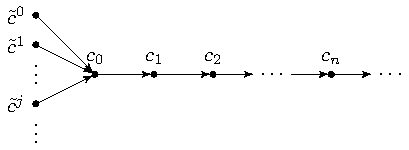
\includegraphics{final-f-infinite-local.pdf}
	\caption{Graphical representation of the ``final'' $f$}
	\label{fig:uai:final-f-sketch}
\end{figure*}

The main idea is to pick a suitable $f$ in $F$ and define the sequence as the iterates $c_{n+1} = f(c_n)$. This function is sketched in Figure~\ref{fig:uai:final-f-sketch}.
The initial set of elements $\tilde{c}^j$ mapped to $c_0$ is required to apply Lemma~\ref{lmm:uai:f-non-repr-pair} to all pairs $\{ \tilde{c}^j, c_n \}$ and get that $c_{n+1} = f(c_n)$ is representable, since $f(\tilde{c}^j) = c_0 \in R$.
The difficulty in realizing this idea is that we do not have enough information on the sequence to pick the right function $f$ at the beginning, so we bring along a list of candidate functions that all coincide on a prefix of the sequence. At step $n$, we pick a new element of the sequence among the possible images of $c_{n-1}$ through all candidate $f$ we have at that point and discard all those functions that cannot match the choice.
Actually, instead of directly considering functions, we represent them with elements $\tilde{c}$ of $C$. Each one represents a function $f_{\tilde{c}}$ that satisfies $f_{\tilde{c}}(\tilde{c}) = c_0$. Note that this can be done for ``enough'' (that is, infinitely many) $\tilde{c}$ because of the high surjectivity hypothesis. We call $E_n$ the set of element $\tilde{c}$ that represent functions that are ``valid'' for the prefix up to $n$, i.e., they map $c_{i}$ to $c_{i+1}$ for $0 \le i \le n - 1$. The core of the proof is an induction that proves that $E_n$ always contains infinitely many elements and that the newly chosen $c_n$ is different from all the previous ones.
\begin{theorem}\label{th:uai:non-empt-res-local}
	Let $F$ be a highly surjective function family from $C$ to itself such that all functions $f \in F$ are either injective or acyclic.
	Assume also that $R\neq \emptyset$. Then there is at least one function $f \in F$ that is not non-emptying in $A$.
\end{theorem}

\begin{remark}
	In the previous section, we developed an ad hoc proof for the family of sums over integers in Proposition~\ref{prop:uai:ne-sum-nonexsistence-inf}, but the same result can also be obtained as an application of Theorem~\ref{th:uai:non-empt-res-local}: if $C = \setZ$ and $F = \{ \lambda x. x + n \svert n \in \setZ \}$, the family is highly surjective (actually $P_F(c) = \setZ$ for all $c$) and all these functions are injective, so it meets the hypotheses of the theorem.
	However, it is interesting to note that the proof of Theorem~\ref{th:uai:non-empt-res-local} is not a generalization of the proof of Proposition~\ref{prop:uai:ne-sum-nonexsistence-inf}. Here we iterate a single $f$ to build the entire sequence, while in the previous one we change the function every time, mapping the non representable $\tilde{n}$ to the newly found representable $n_0 + t d$ to get that the image of $n_0$ through that function is representable too, as sketched in Figure \ref{fig:uai:ne-sum-inf-sketch}.
	\begin{figure*}[ht]
		\centering
		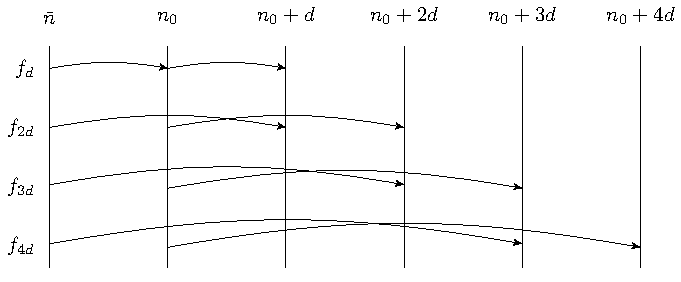
\includegraphics{proof-sum-infinite.pdf}
		\caption{Graphical representation of the proof of Proposition~\ref{prop:uai:ne-sum-nonexsistence-inf}}
		\label{fig:uai:ne-sum-inf-sketch}
	\end{figure*}
\end{remark}

Another example are rational or real numbers, with sums or products.
\begin{example}
	Take $C = \mathbb{Q} \setminus \{ 0 \}$ and $F = \{ \lambda x. x \cdot q \svert q \in \mathbb{Q} \setminus \{ 0 \} \}$.
	The family is highly surjective since $P_F(c) = \mathbb{Q} \setminus \{ 0 \}$ for all $c$, and all these functions are invertible, hence injective.
\end{example}
A possibly more interesting example of application are floating-point numbers as described by the IEEE Standard.
\begin{example}\label{ex:uai:fp-numbers-local}
	Take $C = \mathcal{F} \setminus \{ 0 \}$ the set of non-zero floating-point numbers that can be represented with a fixed number of significant digits, say $t$ bits, but with an arbitrary precision exponent. We choose infinite precision exponents but a finite number of significant digits to have an infinite domain, as required by the theorem, but also to preserve characteristics of floating-point arithmetic.

	Let $\cdot$ and $\odot$ denote respectively real product and its floating-point approximation, and consider the function family $F = \{ \lambda x . x \odot y \svert y \in C \}$. The function family is highly surjective, e.g., considering that all numbers with the same significant digits as a floating-point $x$ but different exponent can be mapped into $x$ by multiplying them by $2$ to the power of the difference of exponents.
	For the second condition, if $y = \pm 1$ we have that the function $\lambda x. x \odot y$ is invertible, hence injective. Otherwise, assume without loss of generality that $y > 1$ (other cases are analogous), and by contradiction assume it has a cycle $f^{n}(x_0) = x_0$. By monotonicity of $\odot$ we have 	$f(x) = x \odot y \ge x \odot 1 = x$, hence $x_0 \le f(x_0) \le f^2(x_0) \le \dots \le f^n(x_0) = x_0$ so all the elements of the cycle are equal, and in particular $f(x_0) = x_0$. However, if $y \neq 1$, the product $x \odot y$ is never equal to $x$, that is a contradiction. Hence the function is acyclic.
	This means $F$ meets the hypotheses of Theorem~\ref{th:uai:non-empt-res-local}, hence no abstract domain on floating-point numbers can be non-emptying for all multiplications.
\end{example}

\subsection{Global requirements for impossibility}
The second set of conditions we propose is ``global'', in the sense that it requires the family $F$ to satisfy a property as a whole.

The proof of this theorem starts from the infinite set $P_F(c_0)$ and, using the hypotheses that some sets are finite, propagates its infiniteness down to $R$, yielding a contradiction with Lemma~\ref{lmm:uai:R-S-bound-integer-inf}, stating that $R$ is finite.
\begin{theorem}\label{th:uai:non-empt-res-global}
	Let $F$ be a highly surjective family of functions  from $C$ to itself such that
	\begin{enumerate}
		\item for all pair of elements $c, d \in C$, the set $\{ f \in F \mid f(d) = c \}$ is finite;
		\item for all pair of an element $c \in C$ and a function $f \in F$, the set $\{ d \in C \mid f(d) = c \}$ is finite.
	\end{enumerate}
	Assume also that $R$ is not empty. Then there is at least one function $f \in F$ that is not non-emptying in $A$.
\end{theorem}

\begin{remark}
	Again, Theorem~\ref{th:uai:non-empt-res-global} can be used to prove Proposition~\ref{prop:uai:ne-sum-nonexsistence-inf}, but the proofs are different.
	The former starts from the infinite set $P_F(c_0) \setminus R(c_0)$ of preimages $\tilde{c}$ of $c_0$ that are not representable with it. This yields an infinite list of pairs $\{ \tilde{c}, c_0 \}$ to apply Lemma~\ref{lmm:uai:f-non-repr-pair}: for any such pair, since $\tilde{c}$ is in $P_F(c_0)$, we get a function $f_{\tilde{c}}$ such that $f_{\tilde{c}}(\tilde{c}) = c_0 \in R$, so that $f_{\tilde{c}}(c_0) \in R$, too. The proof then exploits the remaining hypotheses to prove that there are infinitely many distinct $f_{\tilde{c}}(c_0)$.
	The proof of the latter relies on multiple functions to apply Lemma~\ref{lmm:uai:f-non-repr-pair}, but it always uses the same pair $\{ \bar{n}, n_0 \}$: at every step, it finds a function that maps $\bar{n}$ to the representable element found at the previous step.
\end{remark}

Similarly to Theorem~\ref{th:uai:non-empt-res-local}, this result can be used to prove the impossibility of building an under-approximation abstract domain for floating-point numbers.
\begin{example}\label{ex:uai:fp-numbers-global}
	Take $C = \mathcal{F} \setminus \{ 0 \}$ the set of non-zero floating-point numbers with $t$ bits significands and arbitrary precision exponents, and $F = \{ \lambda x . x \odot z \svert z \in \mathcal{F} \setminus \{ 0 \} \}$.
	As observed in Example~\ref{ex:uai:fp-numbers-local} this family is highly surjective.
	Fixed now two floating-point numbers $x, y$, and letting $\macheps$ be the machine precision of floating-point arithmetic, we have that $y = x \odot z$ only if
	\[
	\left\lvert \frac{y - (x \cdot z)}{x \cdot z} \right\rvert < \macheps
	\]
	that is
	\[
	\left\lvert\frac{y}{x}\right\rvert \frac{1}{1+\macheps} < \abs{z} < \left\lvert\frac{y}{x}\right\rvert \frac{1}{1-\macheps}
	\]
	This is a bounded interval since $x \neq 0$, and hence contains only a finite amount of floating-point numbers. This in turn means that, fixed $x$ and $y$, there is only a finite amount of functions of the form $\lambda x. x \odot z$ such that $f(x) = y$.
	Analogously, fixed a floating-point $y$ and a function $f(x) = x \odot z$, we have that $y = f(x)$ only if $\abs{x}$ belong to a bounded interval, that contains a finite amount of floating-point numbers. So, fixed $y$ and a function $f = \lambda x . x \odot z$, only a finite number of $x$ satisfies $f(x) = y$.
	So, through Theorem~\ref{th:uai:non-empt-res-global} above, we proved again that no abstract domain on floating-point numbers can be non-emptying for all multiplications.
\end{example}

We point out once more that the only hypothesis on the abstract domain is about its size for both theorems in this section. For instance, our result applies to any under-approximation predicate abstraction domain~\cite{GS97}. Such a domain is defined by a (finite) list of predicates, each one representing the set of states satisfying the predicate, and an abstract state is a subset of predicates. By duality with respect to over-approximation, the concretization of such a set is the \emph{union} of the states described by each predicate. Analogously, the abstraction of a set of concrete states $S$ is the set of predicates which are \emph{entirely contained} in $S$. Note that this interpretation is consistent with the use of under-approximations in Incorrectness Logic: the difference is that the logic can use any under-approximation formula, while predicate abstraction is constrained to use just a finite set of predicates, fixed beforehand.

\subsection{On the necessity of high surjectivity}\label{sec:uai:high-surjective}
Both sets of conditions we proposed in this section require the function family to be highly surjective. This turns out to be necessary to prove that no under-approximation abstract domain exists, as we show in this section.

\begin{prop}\label{prop:uai:existence-base}
	For any fixed family $F$ of functions from $C$ to itself that is not highly surjective, there exists an abstract domain $A_F$ for $\pow(C)$ such that:
	\begin{itemize}
		\item $A_F$ is finite, and
		\item all functions $f \in F$ are non-emptying in $A_F$.
	\end{itemize}
\end{prop}

Notably, the above proof is constructive. We present an example of such domain construction below.
\begin{example}\label{ex:uai:construction-ne-domain-base}
	Fix the pair of functions $f(x) = x - 1$ and $g(x) = x - 2$ on $\setZ$. The family $F = \{ f, g \}$ is not highly surjective, so we build an under-approximation abstract domain for which these functions are non-emptying.
	First, take an integer $n_0$ such that $P_F(n_0)$ (computed with respect to $F$) is finite. With this $F$, any integer is a suitable candidate, so let us fix $n_0 = 0$.

	The set of preimages of $0$ is $P_F(0) = \{ 1, 2 \}$. We define the abstract domain $A_F$ as
	\[
	A_F = \{ \emptyset \} \cup \left\lbrace X \cup \{ 0 \} \svert X \subseteq P_F(0) \right\rbrace = \{ \emptyset, \{ 0 \}, \{ 0, 1 \}, \{ 0, 2 \}, \{ 0, 1, 2 \} \} .
	\]
	In this abstract domain, a set is abstracted to $\emptyset$ if and only if it does not contain $0$ since all elements of $A_F$ but $\emptyset$ contains $0$ and the abstraction of a set $S$ must be a subset of $S$.

	To check that $f$ is non-emptying in $A_F$, fix a set $S \subseteq \setZ$. If $\alpha(S) = \emptyset$ the non-emptying condition is vacuously true, so assume this is not the case, or, equivalently, that $0 \in S$. Analogously, if $\alpha(f(S)) = \emptyset$ the condition is true, so assume $0 \in f(S)$ or, equivalently, $1 \in S$. Using these two assumptions we get
	\begin{align*}
		f^{A}(\alpha(S)) & = \alpha(f(\alpha(S)))                  & [\text{def. of }f^{A}]                             \\
		                 & \supseteq \alpha(f(\alpha(\{ 0, 1 \}))) & [\alpha, f \text{ monotone}, S \supseteq \{0, 1\}] \\
		                 & = \alpha(f(\{ 0, 1 \}))                 & [\alpha(\{ 0, 1 \}) = \{ 0, 1 \}]                  \\
		                 & = \alpha(\{ -1, 0 \}) = \{ 0 \}         & [\text{def. of } f \text{ and } \alpha]
	\end{align*}
	The check for $g$ is analogous.
\end{example}
Even though this proposition defines an under-approximation abstract domain, it should not be interpreted as a positive result since the resulting domain is almost a power set and hence too large to be feasible in practice. Instead, the proposition should be regarded as a way to show that one of the hypotheses required in the previous theorems is tight and cannot be weakened. Particularly, since these kinds of results require high surjectivity, they are ill-suited when the focus is on a single function.

This proposition can be generalized to consider sets $S \subseteq C$ whose preimages are finite, but a little care is needed when lifting the definition of preimages to sets of values: a preimage is a set for which there exists a function that maps it to $S$, not the union of the preimages of elements in $S$. Formally, we let:
\[
P_F(S) = \{ T \subseteq C \svert \exists f \in F.~ f(T) = S \} .
\]
Using this definition, we can now easily generalize Proposition~\ref{prop:uai:existence-base}:
\begin{prop}\label{prop:uai:existence-finite-backward}
	Let $F$ be a family of functions from $C$ in itself, and assume there is a set $S_0 \subseteq C$ such that $P_F(S_0)$ is finite. Then there exists a finite abstract domain $A_F$ for $\pow(C)$ such that all functions $f \in F$ are non-emptying in $A_F$.
\end{prop}
This proposition may also be applied to the concrete domain of finite lists to show that a natural function family to consider cannot be used to prove non existence of under-approximation domains using non-emptying functions.
\begin{example}\label{ex:uai:construction-ne-domain-backward}
	Fix the concrete domain $C$ as the set of all lists of finite length over a finite, non-empty alphabet $\Gamma$, i.e. $C = \Gamma^{*}$.
	For $\alpha \in \Gamma^*$ a finite string, let
	\[
	\concat_{\alpha}(\beta) = \alpha \beta
	\]
	be the function that prefixes its argument by the string $\alpha$.
	The family
	\[
	F = \{ \concat_{\alpha} \svert \alpha \in \Gamma^* \}
	\]
	is not highly surjective, because fixed a string $\gamma$ only its suffixes can be mapped into  $\gamma$ by a function in $F$, and they are a finite amount. Hence we can define an under-approximation abstract domain for which all these functions are non-emptying by means of Proposition~\ref{prop:uai:existence-finite-backward}.
	Such domains are defined with a construction similar to that of Example~\ref{ex:uai:construction-ne-domain-base}, and in particular, if $\epsilon$ is the empty list, considering the set $S_0 = \{ \epsilon \}$ whose preimage is only $S_0$ itself, the construction yields
	\[
	A_F = \{ \emptyset, \{ \epsilon \} \} .
	\]
	It is easy to check that all functions $\concat_{\alpha}$ are non-emptying in this abstract domain.
\end{example}

The previous proposition focuses on preimages, stating that if there is a concrete element that has a finite amount of preimages then it is possible to define an under-approximation domain. A natural dual of this proposition can be formulated in terms of images.
For a subset $S \subseteq C$, the set of its images is defined as follows:
\[
I_F(S) = \{ f(S) \svert f \in F \} .
\]
This definition is exactly dual to that of preimages and can be used to formulate a similar result.
\begin{prop}\label{prop:uai:existence-finite-forward}
	Let $F$ be a family of total functions (ie. if $S \neq \emptyset$ then $f(S) \neq \emptyset$) from $\pow(C)$ in itself, and assume there is a non-empty set $S_0 \subseteq C$ such that $I_F(S_0)$ is finite. Then there exists a finite abstract domain $A_F$ such that all functions $f \in F$ are non-emptying in $A_F$.
\end{prop}
Even though Proposition~\ref{prop:uai:existence-finite-forward} introduces the technical hypothesis that all $f \in F$ are total, we don't believe this condition to be very restrictive in practice. Our results are applicable when $F$ is a family of basic transfer functions; in programming languages, non-termination is often due to control-flow constructs, while assignments and guards are usually total.
As an immediate application of the proposition that exploits images instead of pre-images, we consider lists again, and rule out another natural function family.
\begin{example}\label{ex:uai:construction-ne-domain-forward}
	Fix again $C = \Gamma^{*}$, and consider all functions of the form $\dropp_n : \Gamma^* \rightarrow \Gamma^*$ that, taken a list, drop its first $n$ elements and return the resulting list. If the input list is shorter than $n$, the output of $\dropp_n$ is the empty list $\epsilon$.
	The function family
	\[
	F = \{ \dropp_n \svert n \in \setN \}
	\]
	is highly surjective since, for any fixed list $\alpha \in \Gamma^*$ and any $n$, we can prefix $\alpha$ by $n$ arbitrary characters, and map this extended list back to $\alpha$ via $\dropp_n$.
	However, images through this function family are finite:
	\[
	I_F(\alpha) = \{ \dropp_n(\alpha) \svert n \in \setN \}
	\]
	is finite because $I_F(\alpha)$ coincides with the set of all tails of $\alpha$. By Proposition~\ref{prop:uai:existence-finite-forward} we can define an under-approximation abstract domain such that all functions $\dropp_n$ are non-emptying. Again, these domains are constructed from sets $S_0$ with a finite amount of images, and considering $S_0 = \{ \epsilon \}$, that satisfies $I_F(S_0) = \{ \epsilon \}$, we get
	\[
	A_F = \{ \emptyset, \{ \epsilon \} \} .
	\]
	It can be easily checked that all functions $\dropp_n$ are non-emptying in $A_F$.
\end{example}

These last two propositions consider opposite situations in which it is possible to define an under-approximation domain: the former requires to be able to go backward using $F$ in infinitely many ways, while the latter to go forward. This often is not the case in the presence of ``boundaries'' in the concrete domain, which are points with respect to which functions tend to walk either up or away. For instance, $\epsilon$ is such a point with finite lists because $\concat$ functions go away from it while $\dropp$ functions move towards it.
Another example of such a boundary is $0$ in the domain of integers $\setZ$ for multiplications and (rounded) divisions: the former increase absolute value, moving away from $0$ (even though $0$ itself is never a preimage), while the latter decrease it.
Also considering a function family made of both kinds of functions does not work: a slight adaptation of the constructions for the two propositions above shows that, if $F$ can be partitioned into two subfamilies, each satisfying the hypothesis of one of the two propositions, then there exists an under-approximation abstract domain. An example of this is in the set of finite lists, taking as $F$ both $\concat$ and $\dropp$ functions. The construction then yields exactly $A_F = \{ \emptyset, \{ \epsilon \} \}$, for which all these functions are non-emptying, as shown in Examples~\ref{ex:uai:construction-ne-domain-backward} and \ref{ex:uai:construction-ne-domain-forward}.
In light of these observations, to apply the definition of non-emptying function in an effective way for proving the non existence of abstract domains, for all possible boundaries there is the need for a function that can both enter and exit it. This happens for integers since there is no boundary, but does not for finite lists, with $\{ \epsilon \}$ being often either a sink or a source for many functions on lists.

\section{General finite concrete domains}\label{sec:uai:finite}
The discussion of Section~\ref{sec:uai:infinite} requires $C$ to be infinite. While this is a common simplification, since concrete domains have usually a very big size, an interesting and important question is whether our findings can be extended to the case of finite concrete domains.
However, we believe that the two Theorems~\ref{th:uai:non-empt-res-local} and \ref{th:uai:non-empt-res-global} cannot be straightforwardly adapted to the finite setting.

%For both these results, the proof of non existence of the abstract domain was carried out by showing the existence of infinitely many representable elements (defining an infinite sequence in the local result Theorem~\ref{th:uai:non-empt-res-local}, extracting a fraction of the infinite $P_F(c_0)$ in the global Theorem~\ref{th:uai:non-empt-res-global}), against Lemma~\ref{lmm:uai:R-S-bound-integer-inf}. For a finite $C$, if $N = \abs{C}$, one possibility would be to resort to Lemma~\ref{lmm:uai:R-S-bound-integer-fin} to show that $\abs{R} = O(\log(N))$ and get the contradiction by proving the existence of $\omega(\log(N))$ representable elements. Unfortunately, the same and similar constructions do not yield the desired bound: when $C$ is infinite we exploited the fact that finite combinations of finite numbers are also finite, while for finite $C$ we should require that arbitrary combinations of logarithmic factors are $O(N)$, which is not the case.
For both results, the proof showed the existence of infinitely many representable elements, contradicting Lemma~\ref{lmm:uai:R-S-bound-integer-inf}. For a finite $C$, if $N = \abs{C}$, one possibility would be to resort to Lemma~\ref{lmm:uai:R-S-bound-integer-fin} to show that $\abs{R} = O(\log(N))$ and get the contradiction by proving the existence of $\omega(\log(N))$ representable elements (we recall that $f(n) = \omega(g(n))$ if and only if $\lim_{n \rightarrow +\infty} \left( {f(n)} / {g(n)} \right) = +\infty$, which intuitively means that $f$ asymptotically dominates $g$). Unfortunately, similar constructions do not yield the desired bound: when $C$ is infinite we exploited the fact that finite combinations of finite numbers are also finite, while for finite $C$ we should require that arbitrary combinations of logarithmic factors are $O(N)$, which is not true.

The definition of highly surjective family itself is not easy to translate. The construction of Proposition~\ref{prop:uai:existence-base} on a finite $C$ yields an abstract domain with the needed features already when $\abs{P_F(c)} = O(\log(N))$. However, to carry out proofs along the lines of Theorems~\ref{th:uai:non-empt-res-local} and~\ref{th:uai:non-empt-res-global} we would need stronger hypothesis than just $\abs{P_F(c)} = \omega(\log(N))$, possibly up to $\abs{P_F(c)} = \Theta(N)$.

Even with these theoretical considerations against finite counterparts of Theorems~\ref{th:uai:non-empt-res-local} and~\ref{th:uai:non-empt-res-global}, we have been able to carry out the proof for the special case of the finite domain $C = [-N, N]$ of integers (Proposition~\ref{prop:uai:ne-sum-nonexsistence-fin}). Our result exploits the precise structure of both the given concrete domain and function family, particularly two key points.
First, functions produce elements that are not ``too far away'' with respect to the size of the domain (i.e., $n_{i+1} - n_{i} = O(\log(N))$), and this allows to prove that there are enough distinct representable elements.
Second, the domain is circular and hence has no boundaries. If the domain had them, we could have applied results such as Example~\ref{ex:uai:construction-ne-domain-backward} or Proposition~\ref{prop:uai:existence-finite-forward}. This was not the case for integers because additions overflow, so the domain has no boundaries near $-N$ and $N$.

Building on the above discussion, we present a version of the global condition for finite concrete domains. To overcome the limitation of boundaries, we explicitly constrain the initial representable element $c_0$, writing hypotheses around it. Such hypotheses imply that $c_0$ is ``far enough'' from the boundaries of the domain (if any).
Conditions (1-2) of the next theorem correspond to those of the infinite version (Theorem~\ref{th:uai:non-empt-res-global}) rewritten with $c_0$ in mind. The relation between the two bound functions $k_1$ and $k_2$ and the number of preimages of $c_0$ corresponds to the high surjectivity hypothesis. It only constrains the value $c_0$ because this is the representable value from which the proof begins.

As we did in the specific case of the integer domain $[-N; N]$, we assume the size of $A$ to be polynomial in $N$ (Assumption~\ref{assump:uai:size-A-finite-integers}). To say this formally, as we did for finite integers (cfr. Section~\ref{sec:uai:integers-finite}), we consider a sequence $C_N$ of sets of concrete values with size $O(N)$. In the specific instance of integers, such sets were the intervals $[-N; N]$; in general, we require that $C_{N-1} \subseteq C_N$ for all $N$. This inclusion formalizes the intuition that all the $C_N$ are the ``same'' concrete domain instantiated for different sizes.
We also assume to have an abstract domain $A_N$ for each concrete domain $\pow(C_N)$ such that $\abs{A_N} = O(\text{poly}(N))$. As before, we write $R_N$ for $R_{A_N}$, and we remark that Lemma~\ref{lmm:uai:R-S-bound-integer-fin} holds.

\begin{theorem}\label{th:uai:non-empt-res-finite-global}
	Assume $\abs{C_N} = O(N)$, and let $\ugi{\pow(C_N)}{\alpha_N}{A_N}$ be a UGI for all $N$.
	Assume there exists a number $N_1$ and a value $c_0 \in C_{N_1}$ such that, for all $N > N_1$, $c_0$ is representable in $A_N$ (i.e., $c_0 \in R_{N}$).
	Given  two functions $k_1, k_2 : \setN \rightarrow \setN_{>0}$, for any $N$
	let $F_N$ be a family of functions from $C_N$ to itself such that:
	\begin{enumerate}
		\item for all elements $d \in C_N$, $\abs{\{f \in F_N \mid f(c_0) = d \}} \leq k_1(N)$;
		\item for all functions $f \in F_N$, $\abs{\{d \in C_N \mid f(d) = c_0\}} \leq k_2(N)$.
	\end{enumerate}
	Lastly, assume that $\abs{P_{F_N}(c_0)} = \omega(\log(N) \cdot k_1(N) \cdot k_2(N))$.\\
	Then, there exists $N_0$ such that, for all $N > N_0$, it is not possible that all $f \in F_N$ are non-emptying in $A_N$.
\end{theorem}

A straightforward corollary is that, whenever we can verify the hypotheses for all values in $C$, there is no under-approximation domain with a representable element. This is for instance the case for integers and sums, so we recover Proposition~\ref{prop:uai:ne-sum-nonexsistence-fin}:
\begin{example}
	Let $C_N = [-N, N]$ and
	\[
	F_N = \{ \lambda x. x + n (\text{modulo } 2N+1) \svert n \in [-N, N] \} .
	\]

	Fixed any $n_0 \in [-N, N]$, it is easy to check that $P_F(n_0) = [-N, N]$ and $k_1(N) = k_2(N) = 1$. The condition
	\[
	\abs{P_F(n_0)} = \omega(\log(2N + 1) \cdot k_1(2N + 1) \cdot k_2(2N + 1))
	\]
	thus reduces to
	\[
	2N + 1 = \omega(\log(N))
	\]
	that is true. Hence there is no under-approximation abstract domain for integers with at least one integer $n_0$ representable and that makes all sums non-emptying.
\end{example}
The example of integers has the nice property of not having boundaries, but this is seldom the case. For instance, consider floating point numbers: they overflow and underflow to special values, hence they do have boundaries. Nevertheless, if we pick a suitable initial element $c_0$ we can still apply the theorem above.

\begin{example}
	Consider the finite set of non-zero floating-point numbers $C = \mathcal{F} \setminus \{ 0 \}$ with $t$ bits significand, one bit sign and $e$ bit exponents.
	Consider the function family $F = \{ \lambda x . x \odot z \svert z \in \mathcal{F} \setminus \{ 0 \} \}$ of floating-point multiplications, where $\odot$ denotes the floating-point approximation of real product.

	As shown in Example~\ref{ex:uai:fp-numbers-global}, fixed two floating-point numbers $x, y$, we have that $y = f(x) = x \odot z$ only if
	\[
	\abs{z} \in \left[ \left\lvert\frac{y}{x}\right\rvert \frac{1}{1+\macheps}, \left\lvert\frac{y}{x}\right\rvert \frac{1}{1-\macheps} \right] .
	\]
	If $\macheps \le 1 / 2$ this is entirely contained in the interval
	\[
	\left[ \left\lvert\frac{y}{x}\right\rvert (1 - 2 \macheps), \left\lvert\frac{y}{x}\right\rvert (1 + 2 \macheps) \right] \text{.}
	\]
	It can be shown that, if $\macheps < 1 / 2$, the quantity of floating point numbers in that interval is bounded by a constant $c$ that does not depend on $x$ and $y$.\footnote{For instance, this can be proved for $c = 17$.}
	Analogously, fixed $y$ and $z$ there are at most $c$ floating point numbers $x$ such that $y = f(x) = x \odot z$.

	With these two bounds, if $x_0$ has enough preimages we can verify the last hypothesis of the theorem: letting $N = \abs{C}$
	\[
	\abs{P_F(x_0)} = \omega(\log(N) \cdot k_1(N) \cdot k_2(N)) = \omega(\log(N) \cdot c \cdot c) = \omega(\log(N)) .
	\]
	For instance $x_0 = 1$ satisfies this condition (more than half of all floating-point numbers have a floating-point inverse, hence $\abs{P_F(x_0)} \ge N / 2 = \Theta(N)$) but there are many other points satisfying it.
	By mean of Theorem~\ref{th:uai:non-empt-res-finite-global}, no under-approximation abstract domain is non-emptying for all multiplications whenever one of these points is representable.
\end{example}

\section{Summary}
In this chapter, we pointed out some asymmetries between over and under-approximation in Abstract Interpretation, and why those are an obstacle to the design of abstract domains for program analysis via under-approximation Galois connections. The key observation is that the duality between under and over-approximation is broken by the fact that in program analysis over and under-approximations have to be applied to the same transfer functions. The handling of divergence in the abstract domain poses another critical issue.

Building on those ideas, we proposed the novel definition of \emph{non-emptying function} and studied how it plays a crucial role in proving the non-existence of general, useful under-approximation based abstract domains. Indeed, our results prove that an analysis based on such domains will very often answer $\bot$ (representing either absence of information or divergence) for programs that require repeated applications of non-emptying functions. This is a big limitation since recovery from $\bot$ in an under-approximation is not as easy as recovering from $\top$ in an over-approximation: we can say that it is quite impossible.
We applied our general results to several concrete domains to conclude that, under some mild assumptions, there are no useful under-approximation abstract domains for program analysis. Then, to show that one of the hypotheses in our result is tight, we proposed a construction to craft an under-approximation abstract domain whenever such a hypothesis is not met.

To summarize, our results hint at the difficulty of designing under-approximation abstract domains. This suggest that it is better to resort to other under-approximation techniques to combine with over-approximation ones, including usual over-approximation abstract interpretation domains. Therefore, in the next chapter we study logical frameworks for under-approximation.
